\chapter{Monte Carlo radiation transport technique}
\label{sec:mcrt}
\section{Introduction and Background}
This chapter will provide an overview of the Monte Carlo method and how it is used within the context of \gls{mcrt}. The chapter will then present the details of the MCRT code used as the basis of the subsequent chapters. Validation of this code and details of computational speed up are also presented. Subsequent chapters will expand upon the code for each individual projects needs.

\subsection{Monte Carlo method}\label{sec:mcmethod}
The Monte Carlo method is a numerical analysis technique based upon random numbers, which are used to calculate unknown variables in problems. 

The earliest use of the method is in Buffon's needle experiment of the 18$^{th}$ century~\cite{badger1994lazzarini,beckmann2015history,buffon1785histoire}. Buffon asked the question;

\medskip

``Suppose we have a floor made of parallel strips of wood, each the same width, and we drop a needle onto the floor. What is the probability that the needle will lie across a line between two strips?"

\medskip

The solution to this question is as:
for a needle length \textit{l}, strip separation \textit{s}, and where \textit{x} is the distance from the needle to the closest line. Then using a simple geometrical argument, a needle crosses a strip if $x \leq \tfrac{l}{2} sin \theta$.

$x$ is distributed uniformly in [0, $\tfrac{s}{2}$], and $\theta$ in [0, $\tfrac{\pi}{2}$]. Therefore the probability density function for $x$ is $p(x)=\tfrac{2}{s}$, and $\theta$ is $p(\theta) = \tfrac{2}{\pi}$. The \gls{pdf}, is a function of a variable that gives probability for a variable to a take a given value. The \gls{pdf} is normalised over the whole range of the variable, in this case $x$, and $\theta$.
Thus, as $x$ and $\theta$ are independent variables, giving a joint probability of $p(x,\theta) = \tfrac{4}{s \pi}$.
So the probability of a needle of length l ($l<s$) is:

\begin{equation}
P=\int_0^{\frac{\pi}{2}}\int_0^{\frac{l}{2}sin\theta}\frac{4}{s\pi}dx d\theta = \frac{2 l}{s \pi}\label{eqn:buffon}
\end{equation}


\Cref{eqn:buffon} can be used to carry out a Monte Carlo estimation of pi. A simple rearrangement yields: $\pi = \tfrac{2l}{sP}$ where P is the ratio of needles crossing the line over total number dropped. Laplace was the first to suggest that Buffon's needle experiment could be used to estimate $\pi$~\cite{beckmann2015history}. \Cref{fig:buffon-needle} shows an example of simulation of Buffon's needle experiment.

\begin{figure}
\centering
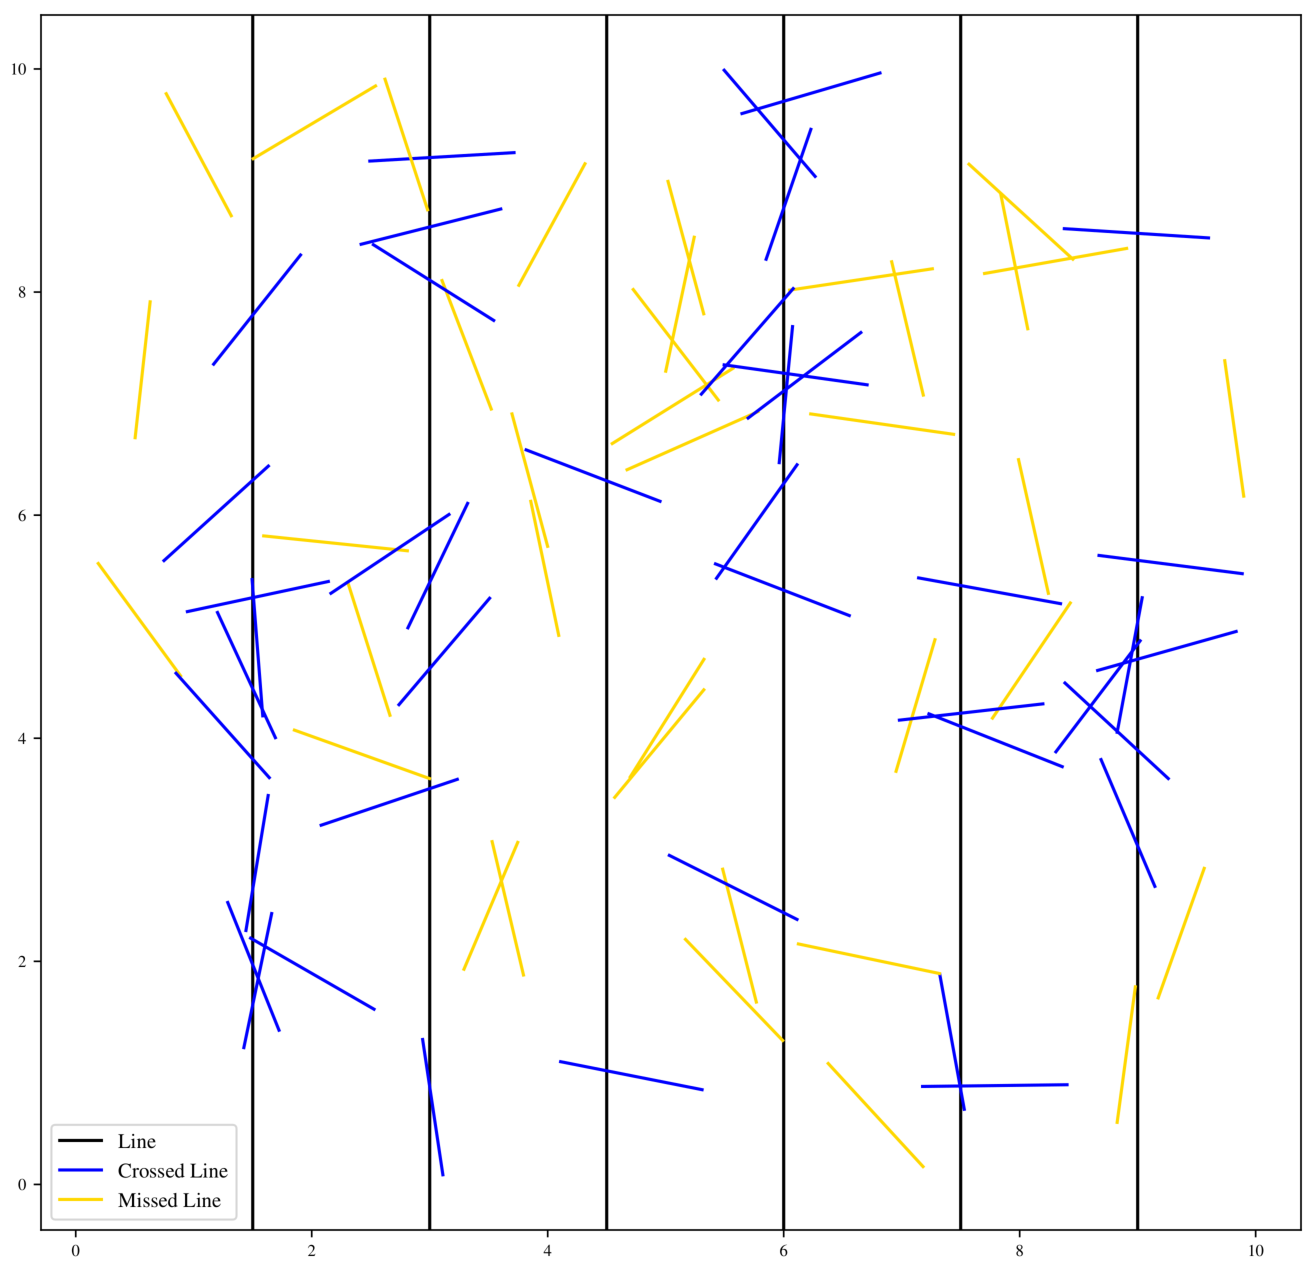
\includegraphics[width=\columnwidth/2]{buffon-pi=317.pdf}
\caption{Sample buffon needle experiment. 100 needles are dropped on a 10 by 10 cm area with lines spaced 1.5cm apart. If a needle lands on a line it is recorded and colored blue, else it is yellow. This simulation gave a value of pi as 3.17.}
\label{fig:buffon-needle}
\end{figure}

The Monte Carlo method is used in various different disciplines. Ranging from use in the financial sector to analyse investments and stocks by simulating the sources of uncertainty which affect their values~\cite{jackel2002monte,finaceprrof}, use in statistical analysis~\cite{wall2012practical}, and in modern computer generated images (see \cref{fig:ray-trace})~\cite{Kajiyarendering,Cookraytracing}.

\begin{figure}
\centering
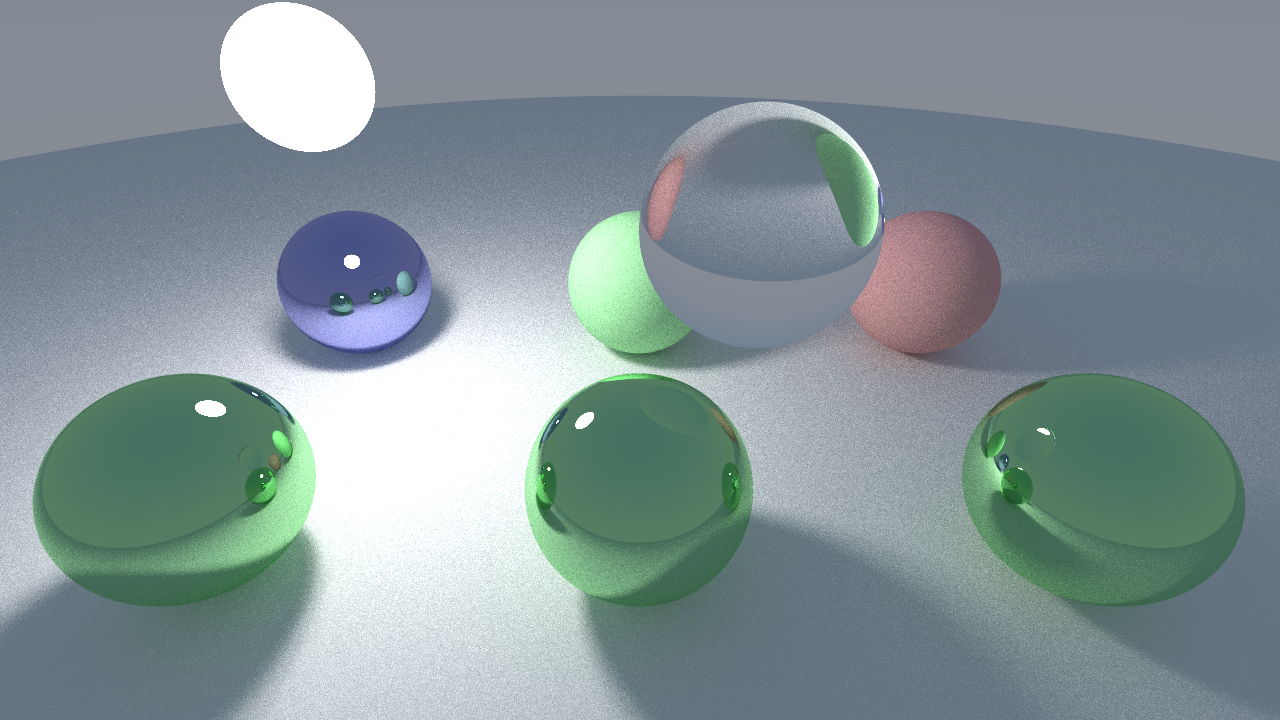
\includegraphics[width=\columnwidth]{ray-tracing.png}
\caption{Computer generated imagery using ray-tracing. Code usd to create image available at: \url{https://github.com/lewisfish/RayTran}}
\label{fig:ray-trace}
\end{figure}

\section{Monte Carlo radiation transport algorithm}

\subsection{Introduction $\&$ background}
The technique that makes up the bulk of this thesis, is the \gls{mcrt} technique. This method was developed at the tail end of World War two at the Los Alamos National Laboratory, for the purpose of calculating neutron diffusion though shielding material~\cite{montybeg1,eckhardt1987stan,anderson1986metropolis,ulam1947statistical}. It has since found a myriad of applications from light transport through dusty clouds~\cite{wood1999model}, calculating doses for radiotherapy~\cite{rogers1995beam} to light transport through tissue~\cite{1stmonty}.

\subsection{MCRT algorithm}

The \gls{mcrt} algorithm can be as simple as a $\sim$ 20 line program to as complex as needed for the problem at hand. This section will provide a detailed description a simple \gls{mcrt} algorithm for a 3D voxel based grid.

\subsubsection{Grid set-up}\label{sec:photsetup}

The first step of the \gls{mcrt} algorithm is to set-up the grid which acts as the simulated medium. This grid consists of $n \times n \times n$ voxels\footnote{A voxel is a 3D pixel} of which each voxel has it's own optical properties. This allows the medium of interest to be discretised onto a grid, which gives a good approximation of the real-life medium (see~\cref{sec:codefurther} for discussion on this). Once the medium has been set-up photon packets are launched and propagated through the voxel structure.


%\begin{figure}
%\centering
%\caption{test}\label{fig:voxeldemo}
%\end{figure}

\subsubsection{Photon launch}\label{sec:photlaunch}

The initial step of any \gls{mcrt} algorithm is to launch a photon packet. Depending on the source of photon packets for a given simulation, this step varies from simulation to simulation. The general idea of launching a photon packet is that the packet is given an initial direction vector and position (which consists of a physical position and a voxel position)\footnote{all variables given in this section are the same as they are in the code.}:

\begin{align}
	direction &= \begin{bmatrix}
		n_{xp}\\
		n_{yp}\\
		n_{zp}
	\end{bmatrix}\\
	position &= \begin{bmatrix}
		x_p, y_p, z_p\\
	\end{bmatrix}\\
	voxel &= \begin{bmatrix}
		x_{cell}, y_{cell}, z_{cell}
	\end{bmatrix}	 
\end{align}

In order to set the direction vectors, the components of the direction vectors must be first set. The packets position is tracked using a Cartesian coordinate system, however for ease of computation for calculating scattering angles (see~\cref{sec:photscatterabsorb}), the direction vectors are computed in a spherical system thus the direction vectors are: 

\begin{align}
n_{xp} &= sin(\theta) \cdot cos(\phi) \\
n_{yp} &= sin(\theta) \cdot sin(\phi) \\
n_{zp} &= cos(\theta)
\end{align}

$\theta$ and $\phi$ are generated dependant on the photon source used.

\subsubsection{Photon move}\label{sec:photmove}

The next step in the algorithm is moving a packet to the next interaction point. The probability a packet will interact over a distance $dL$ is $\mu_tdL$, where $\mu_t$ is the interaction probability (see~\cref{sec:optprop}). Thus the probability of travelling $dL$ without any interaction is $1-\mu_tdL$. Therefore over a distance $L$, with N segments of length $L/N$ the probability of travelling $L$ before any interaction:

\begin{align}
P(L) &= (1-\mu_t\frac{L}{N}) \cdot (1-\mu_t\frac{L}{N}) ...\ (1-\mu_t\frac{L}{N}) = (1-\mu_t\frac{L}{N})^N \\
P(L) &= \lim_{N \to \infty}(1-\mu_t\frac{L}{N})^N=e^{-\mu_tL}=e^{-\tau}\label{eqn:pdfdist}
\end{align}

Where $\tau$ is the number of mean free paths over a distance L. We now have a \gls{pdf}, \cref{eqn:pdfdist}, for the distance a packet will travel before an interaction occurs. For this to be of use we need to be able to sample from this \gls{pdf} in order to get a random optical depth. Using the Monte Carlo method described in~\cref{sec:mcmethod}, with $\xi$ as our random variable, we get:

\begin{equation}
\xi=\int_{0}^{\tau}e^{-\tau'}=1-e^{-\tau}\rightarrow \tau=-log(1-\xi)
\end{equation}

As $\xi$ is symmetric about 0.5 we can substitute $1-\xi$ for $\xi$ yielding:

\begin{equation}
\tau=-log(\xi)\label{eqn:taueqn}
\end{equation} 

We now have an optical distance, however we need to convert this into a physical distance so that we can move our photon packet. From our definition of $\tau$ we know that $\tau=\int_0^L\mu_tdS$, and if we have a smooth, homogeneous medium (i.e not a gridded medium) thus 

\begin{equation}
L=\frac{\tau}{\mu_t}\label{eqn:physicaldist}
\end{equation}

Therefore in order to update the packets position is simply:

\begin{align}
x_p &= x_p+L\cdot n_{xp}\label{eqn:update1}\\
y_p &= y_p+L\cdot n_{yp}\label{eqn:update2}\\
z_p &= z_p+L\cdot n_{zp}\label{eqn:update3}
\end{align}

However as the code in this thesis is a 3D gridded Cartesian code, we have to slightly adjust how we move and update the packets position. As stated in~\cref{sec:photsetup}, the medium has been discretised onto a grid, so that each voxel can have a different $\mu_t$, thus~\cref{eqn:physicaldist} becomes:

\begin{equation}
L=\frac{\tau}{\mu_{t,\zeta}}\quad\quad \zeta=(x,y,z)
\end{equation}

with $\mu_{t,\zeta}$ the $\mu_t$ for the $\zeta^{th}$ voxel. The position is then updated as before using~\cref{eqn:update1,eqn:update2,eqn:update3}. The next step in the algorithm is the interaction event, which can consist of either: scattering, absorbing or fluorescing.

\subsubsection{Photon scatter and absorbing}\label{sec:photscatterabsorb}

The first part of this section of the algorithm is to decide what kind of interaction the packet has with the medium. This section will focus on scattering and absorbing with other interaction events left for the chapters that detail these behaviours.
\medskip

To decide whether a packet scatters or absorbs involves `throwing' a random number and comparing it against the albedo. As detailed in~\cref{sec:optprop} the albedo is the scattering probability $a=\tfrac{\mu_a}{\mu_a+\mu_s}$. The random number is compared to the albedo, and if the random number is less than the albedo then the packet scatters, otherwise the packet is absorbed.

\paragraph{Packet absorption}\hspace{0pt}\\
\\
If the interaction event is a photon packet absorption, then the algorithm terminates the photon packets and starts the next photon packet,~\cref{sec:terminator}.

\paragraph{Packet scattering}\hspace{0pt}\\
\\
If the interaction event is a packet scattering, then the packet is scattered into a new direction and the above process are carried out until a termination clause is met, see~\cref{sec:terminator}.

Depending of the medium being simulated, it can either be isotropically scattering or preferentially scattering in a direction. In the case of simulating photon propagation in tissue, tissue is highly forward scattering.

Anisotropy is the degree of deviation in the photon packets path at each interaction event. The measure of anisotropy is the g value, $g$. With $g$ taking any value from $-1$ to $1$, $-1$ is highly backward scattering, $0$ is isotropic scattering and $1$ is highly forward scattering. 


\subsubsection{Termination}\label{sec:terminator}

\subsection{Code details}

This section details the the actual implementation of the \gls{mcrt} algorithm detailed in the previous section, along with any computational necessities and speed ups on the original algorithm.

\section{Validation of MCRT code}
\section{Optical properties}\label{sec:optprop}
\section{Further extensions to the code}\label{sec:codefurther}